% This text is proprietary.
% It's a part of presentation made by myself.
% It may not used commercial.
% The noncommercial use such as private and study is free
% Sep. 2005 
% Author: Sascha Frank 
% University Freiburg 
% www.informatik.uni-freiburg.de/~frank/
%
% additional usepackage{beamerthemeshadow} is used
%  
%  \beamersetuncovermixins{\opaqueness<1>{25}}{\opaqueness<2->{15}}
%  with this the elements which were coming soon were only hinted
\documentclass{beamer}
%\usetheme{bars}
\usepackage{beamerthemeshadow}
\begin{document}
\title{Offline Handritting Word Recognition}  
\author{Thijs Kooi, Davide Modolo}
\date{\today} 

\frame{\titlepage} 

\frame{\frametitle{Table of contents}\tableofcontents} 

% SECTION: OVERVIEW OF THE PROJECT
\section{Overview}

\frame{
\begin{beamerboxesrounded}{}
\centering Overview of the Project
\end{beamerboxesrounded}
}
\subsection{General}
\frame{\frametitle{Off-line handwriting recognition}  
\begin{itemize}
\item It involves the automatic conversion of text in an image into letter codes which are usable within computer and text-processing applications
\item Off-line handwriting recognition is comparatively difficult, as different people have different handwriting styles

\begin{figure}
  \centering
    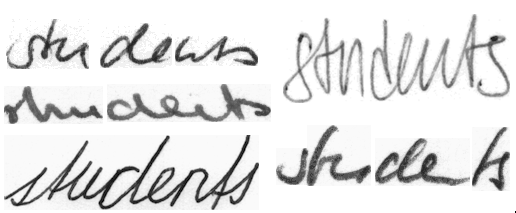
\includegraphics[width=0.5 \textwidth]{Images/studs.png}
   \caption{'Students' written by different authors}
   \label{fig:student}
\end{figure}
\end{itemize}
}

\frame{\frametitle{Our AI Project}
A lot of research has been done over the past years.\vspace{\baselineskip}

We explored the topic and implemented a full pipeline for the task.
The research touched different fields:
\begin{itemize}
\item Data Collection
\item Image Processing
\item Features extraction 
\item Machine Learning 
\item Word Recognition
\end{itemize}
}

\subsection{Dataset}
\frame{\frametitle{Dataset}
The IAM Handwriting Database 3.0\footnote{http://www.iam.unibe.ch/fki/databases/iam-handwriting-database}  \vspace{\baselineskip}

\begin{itemize}
%\item It contains forms of handwritten English text which can be used to train and test handwritten text recognizers and to perform writer identification and verification experiments.
\item Unconstrained handwritten text (scanned at a resolution of 300dpi and saved as PNG images with 256 gray levels) 
\item 1'539 pages of scanned text of 657 writers
\item 13'353 isolated and labeled text lines
\item 115'320 isolated and labeled words
\end{itemize}
}

\frame{\frametitle{Example of a page of scanned text}  
\begin{figure}
  \centering
    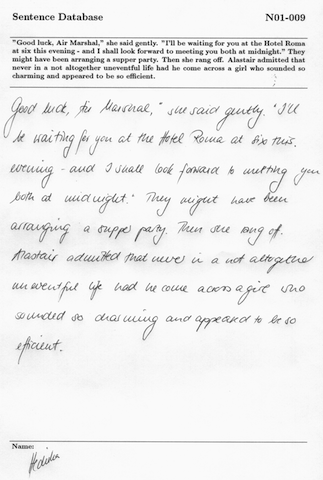
\includegraphics[width=0.5\textwidth]{Images/database.png}
   \caption{Example of page of scanned text}
   \label{fig:dataset}
\end{figure}
}


%SECTION: IMPLEMENTATION DETAILS
\section{Implementation Details}
\frame{
\begin{beamerboxesrounded}{}
\centering Implementation Details
\end{beamerboxesrounded}
}

\subsection{Pipeline}
\frame{\frametitle{Pipeline}  
\begin{figure}
  \centering
    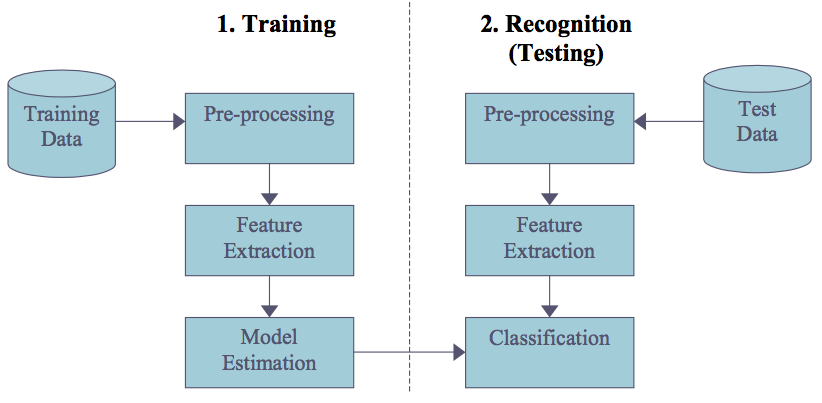
\includegraphics[width=1.02 \textwidth]{Images/pipeline.png}
   \caption{Pipeline of a word recognition system}
   \label{fig:pipeline}
\end{figure}
}

\subsection{Pre-Processing}
\frame{
\begin{beamerboxesrounded}{Implementation Details}
\centering Pre-Processing
\end{beamerboxesrounded}
}

\frame{\frametitle{Pre-processing}  
\begin{figure}
  \centering
    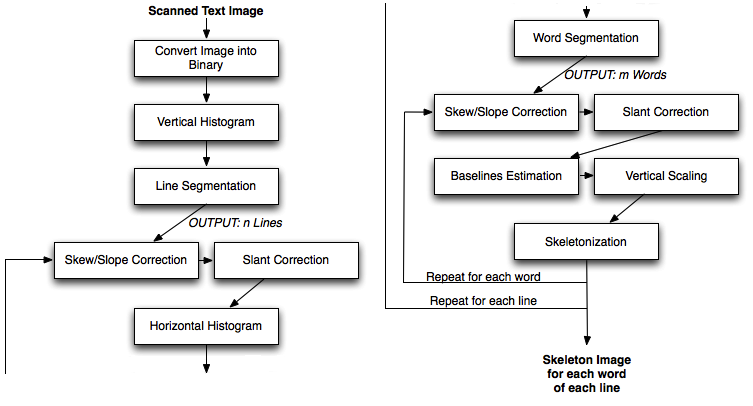
\includegraphics[width=1\textwidth]{Images/pipelinePP.png}
   \caption{Pipeline for the pre-processing/normalization step}
   \label{fig:pipeline}
\end{figure}
}



\frame{\frametitle{Line Segmentation}  
\begin{figure}
  \centering
    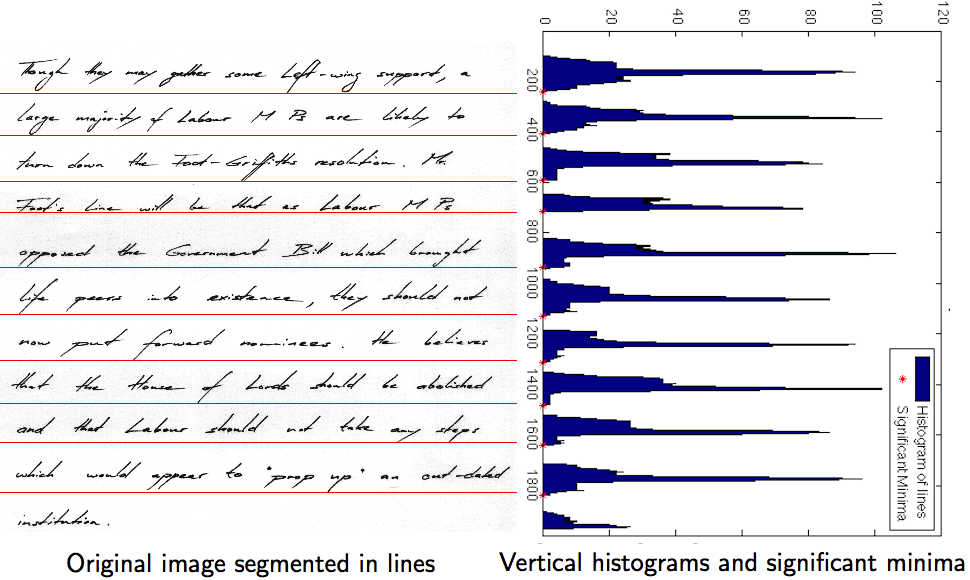
\includegraphics[width=0.93 \textwidth]{Images/line_segmentation.png}
   \caption{Example of line segmentation}
   \label{fig:lineSegm}
\end{figure}
}


\frame{\frametitle{Skew and Slope Correction}  
\begin{figure}
  \centering
    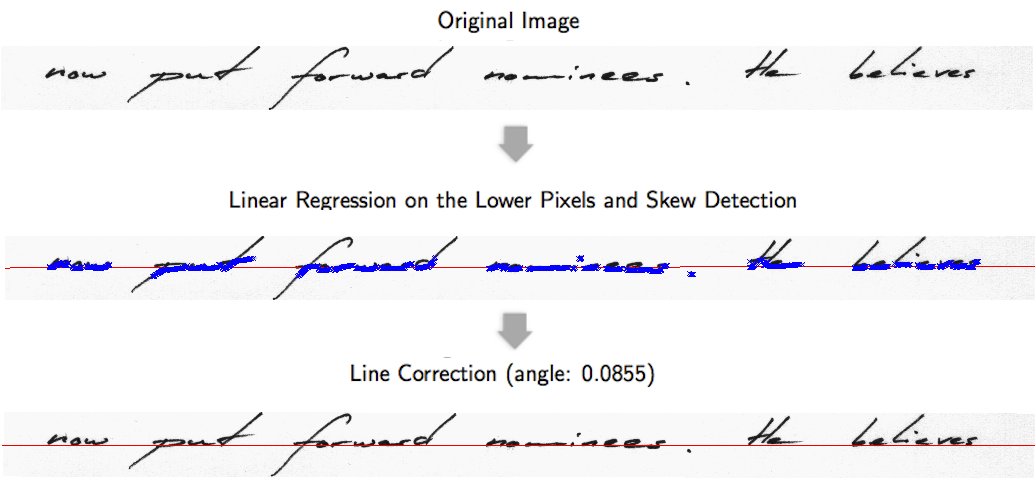
\includegraphics[width=1.0 \textwidth]{Images/skew.png}
   \caption{Skew detection and correction pipeline}
   \label{fig:skew}
\end{figure}
}


\frame{\frametitle{Slant Correction}  
\begin{figure}
  \centering
    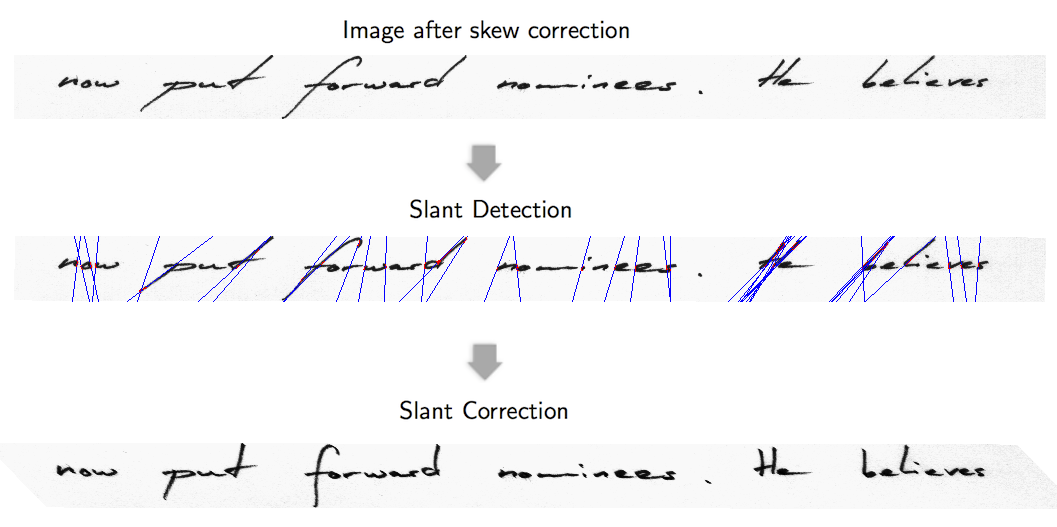
\includegraphics[width=1 \textwidth]{Images/slant.png}
   \caption{Slant detection and correction pipeline}
   \label{fig:slant}
\end{figure}
}

\frame{\frametitle{Word segmentation}
\begin{figure}
  \centering
    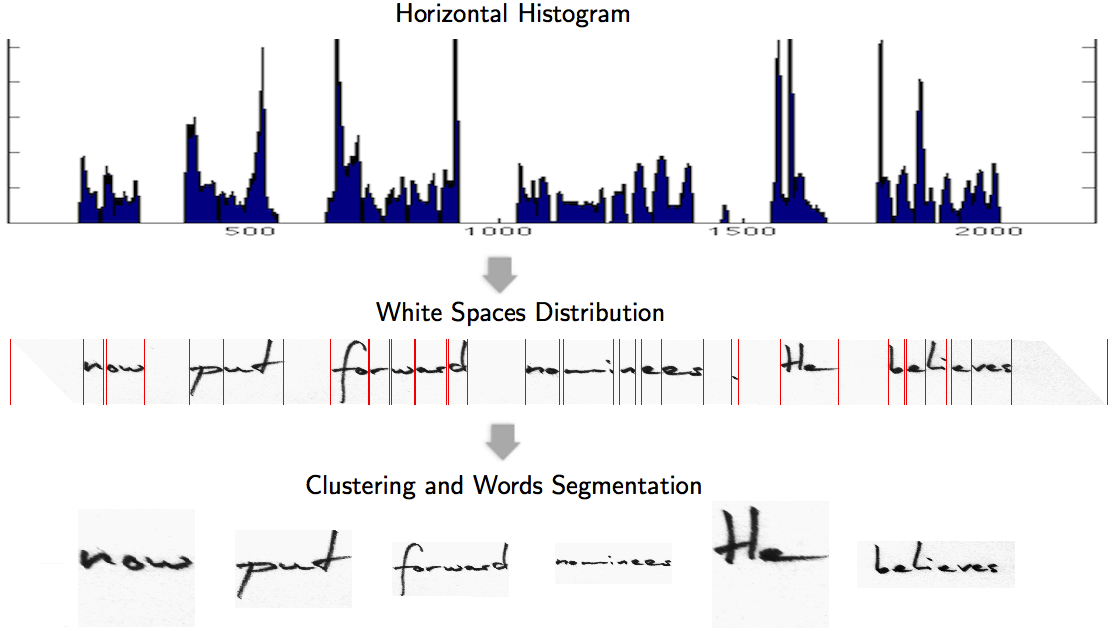
\includegraphics[width=1.0 \textwidth]{Images/word_segmentation.png}
   \label{fig:words_res}
\end{figure}
}  

\frame{\frametitle{Baseline Estimation}
\begin{figure}
  \centering
    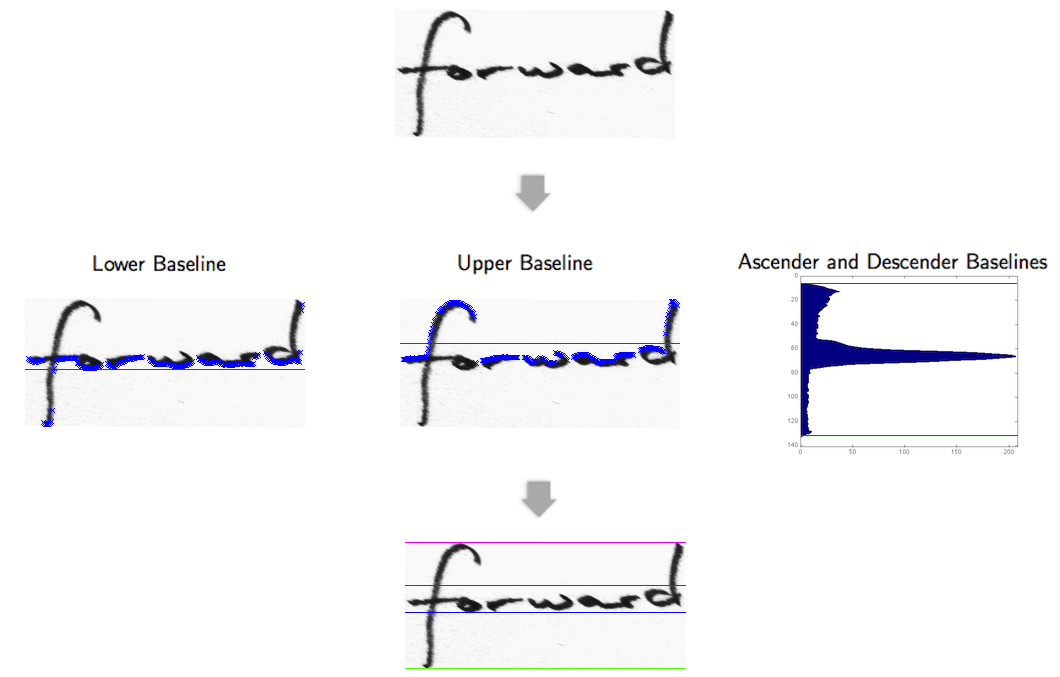
\includegraphics[width=0.95 \textwidth]{Images/baseline.png}
   \label{fig:baselines}
\end{figure}
}  

\frame{\frametitle{Vertical Scaling}
\begin{figure}
  \centering
    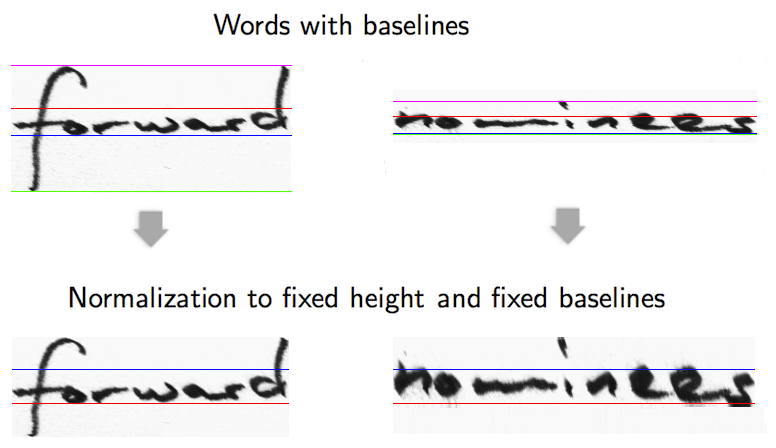
\includegraphics[width=0.90 \textwidth]{Images/vertical_scaling.png}
   \label{fig:scal}
   \caption{Examples of vertical scaling process}
\end{figure}
}  

\frame{\frametitle{Skeletonization}
\begin{figure}
  \centering
    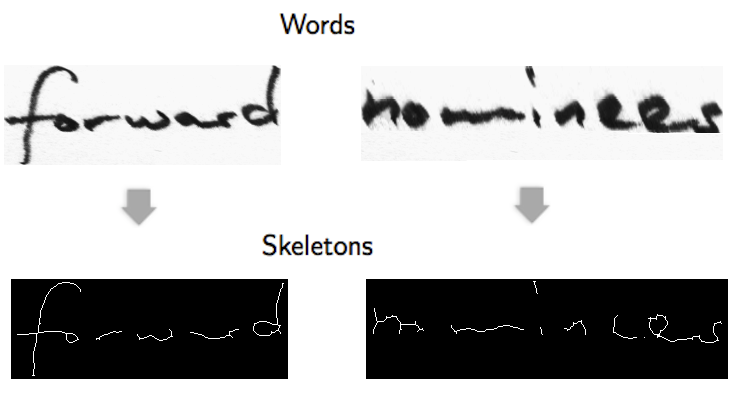
\includegraphics[width=0.90 \textwidth]{Images/skeleton.png}
   \label{fig:skel}
   \caption{Skeletonization process}
\end{figure}

}  

\frame{\frametitle{Remembering the entire pipeline....}
 \begin{beamerboxesrounded}{}
\centering \bf{Why repeating skew and slant correction twice?}
\end{beamerboxesrounded}
\begin{figure}
  \centering
    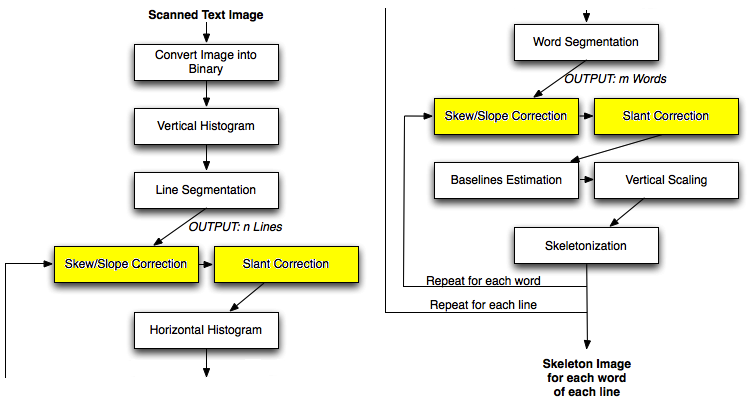
\includegraphics[width=1\textwidth]{Images/pipelinePPex.png}
   \label{fig:pipelineEx}
\end{figure}
}  

\frame{\frametitle{The normalizations are necessary for:}
 \begin{beamerboxesrounded}{First}
%  \begin{itemize}
%\item 
Words segmentation 
 %\end{itemize}
\begin{figure}
  \centering
    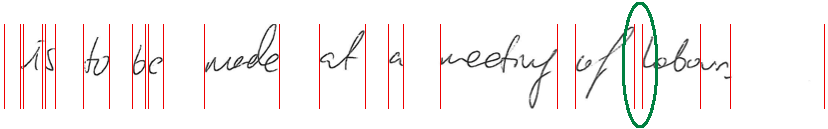
\includegraphics[width=0.9\textwidth]{Images/problem1.png}
   \label{fig:problem1}
\end{figure}
\end{beamerboxesrounded}

 \begin{beamerboxesrounded}{Second}
 %\begin{itemize}
%\item 
Not all the words have the same slope, slant and lower baseline
 %\end{itemize}
\begin{figure}
  \centering
    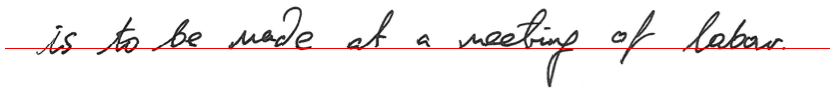
\includegraphics[width=0.9\textwidth]{Images/problem2.png}
   \label{fig:problem2}
\end{figure}

\end{beamerboxesrounded}


}  





\subsection{Feature Extraction}
\frame{
\begin{beamerboxesrounded}{Implementation Details}
\centering Feature Extraction
\end{beamerboxesrounded}
}

\frame{\frametitle{Features}  

Extracted from the skeleton of the words. \vspace{\baselineskip}

Mainly 2 types:
\begin{itemize}
\item Statistical
\item Morphological
\end{itemize}
}

%  We want to find features that minimize the within-class variability and maximize the between class variability. On top of this, the features should be robust against distortions caused by different handwriting styles. Moreover, we want to find low dimensional feature vectors and would therefore like features to be highly descriptive.
%  The selection of features depends both on the pre-processing and the classifier to use. If all characters are assumed to have the same orientation, we need rotation variant features to distinguish between for instance a 6 and a 9 and a b and an p, etc.
  

\frame{\frametitle{Statistical Features}  
Percentage of white pixels in the 3 zones of the word:
\begin{figure}
  \centering
    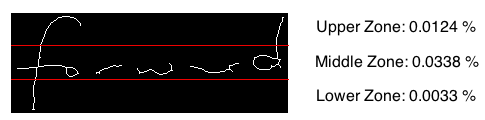
\includegraphics[width=0.8\textwidth]{Images/statisticalFeatures.png}
   \label{fig:statFeatures}
   \caption{Example}
\end{figure}
}

\frame{\frametitle{Morphological Features}  
Obtained by {\bf connected component analysis}.

\begin{itemize}
\item A connected component it is a subgraph in which any two vertices are connected to each other by paths, and which is connected to no additional vertices.
\end{itemize}

\begin{figure}
  \centering
    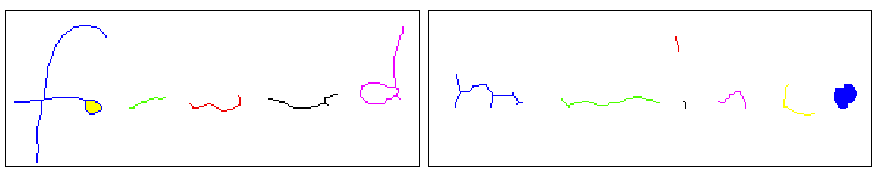
\includegraphics[width=0.9\textwidth]{Images/components.png}
   \label{fig:comp}
   \caption{Example of words divided in different components (colors)}
\end{figure}
}

\frame{\frametitle{Morphological Features}  
We extract:
\begin{figure}
  \centering
    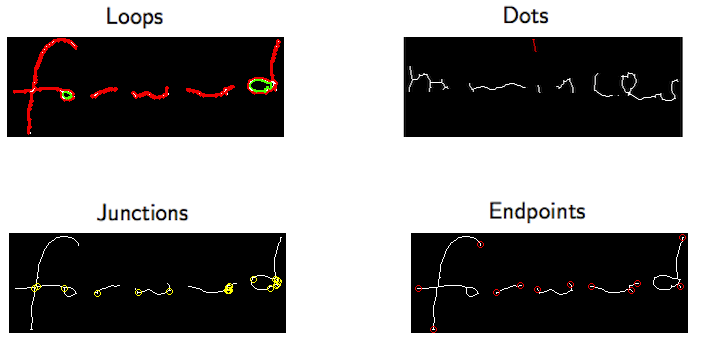
\includegraphics[width=1 \textwidth]{Images/morpho_features.png}
   \label{fig:morphFeatures}
\end{figure}
}

\subsection{Hidden-Markov Model}
\frame{\frametitle{HMM}
  \begin{itemize}
  \item A set of $N$ states $S = (s_{1}, s_{2}, \ldots, s_{N})$, where the state of the system at time $t$ is denoted $q_{t}$
  \item A set of priors ${\bf \pi} = (\pi_{1}, \pi_{2}, \ldots, \pi_{N})$, providing the probability $P(q_{1} = s_{i})$.
  \item A transition function ${\bf A}$, where $a_{ij} = P(q_{t+1} = s_{j} | q_{t} = s_{i})$. 
  \item An observation function ${\bf B}$, mapping each observation at every state to a probability $b_{i}({\bf o}_{t}) = P({\bf o}_{t} | q_{t} = s_{i}, \lambda)$, where $\lambda$ denotes the model parameters.
  \end{itemize}
  The model is trained to estimate the posterior probability $P({\bf O}|\lambda)$ of an observation sequence ${\bf O}$, with $D$-dimensional observation vectors ${\bf o}_{t} = (o_{1},o_{2},\ldots,o_{D})$.
}

\frame{\frametitle{HMM}  

  \begin{figure}
  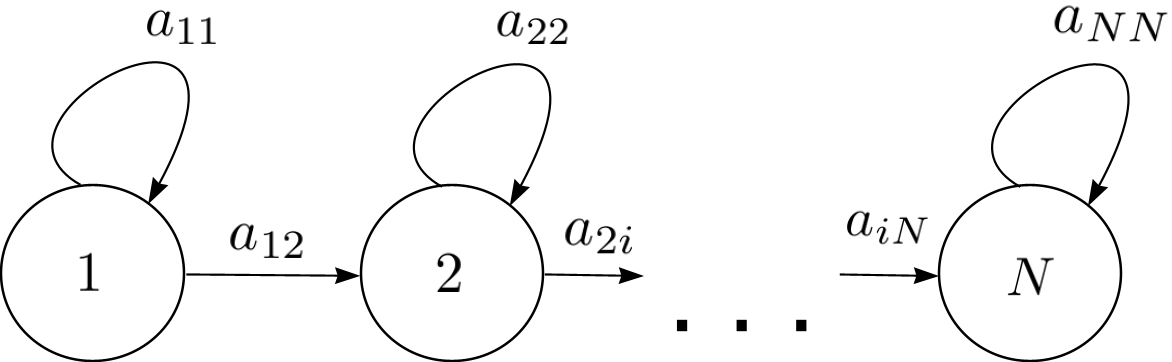
\includegraphics{hmm.jpg} 
  \caption{Left-to-right HMM with N states}
  \end{figure}

}

\frame{\frametitle{Main problems in an HMM}
  \begin{enumerate}
 \item The probability of an observation sequence, given the model, $P({\bf O}|\lambda)$.
 \item The most likely parameters of the model $\lambda^* = \max P(X|\lambda)$, given a training set of $M$ observation sequences $X = ({\bf O}_{1}, {\bf O}_{2}, \ldots, {\bf O}_{M} )$.
  \item The most likely state sequence, underlying a given observation sequence and the model, $Q^* = \max P(Q|{\bf O},\lambda)$.
\end{enumerate}
}

\frame{\frametitle{Main problems in an HMM}
  \begin{enumerate}
 \item The probability of an observation sequence, given the model, $P({\bf O}|\lambda)$.
 \begin{beamerboxesrounded}{}
   Sum-product algorithm: forward-backward algorithm
\end{beamerboxesrounded}
	
 \item The most likely parameters of the model $\lambda^* = \max P(X|\lambda)$, given a training set of $M$ observation sequences $X = ({\bf O}_{1}, {\bf O}_{2}, \ldots, {\bf O}_{M} )$.
  \begin{beamerboxesrounded}{}
  EM-algorithm: Baum-Welch reestimation
\end{beamerboxesrounded}
      
\item The most likely state sequence, underlying a given observation sequence and the model, $Q^* = \max P(Q|{\bf O},\lambda)$.
  \begin{beamerboxesrounded}{}
  Dynamic programming: Viterbi algorithm
\end{beamerboxesrounded}

\end{enumerate}
}

\frame{\frametitle{Forward probability}
\begin{columns}
 
\column{1.5in}
\[
 \alpha_{t}(i) \equiv
\]
\[
  P(o_{1},o_{2},\ldots, o_{t}| q_{t} = s_{i}, \lambda) = 
\]
\begin{equation}
 \label{forwardProbability}
\displaystyle \Big [ \sum_{j=1}^{N}  \alpha_{t-1}(j) a_{ij} \Big ] b_{j}(o_{t})
\end{equation}
\column{2in}
  \begin{figure}
  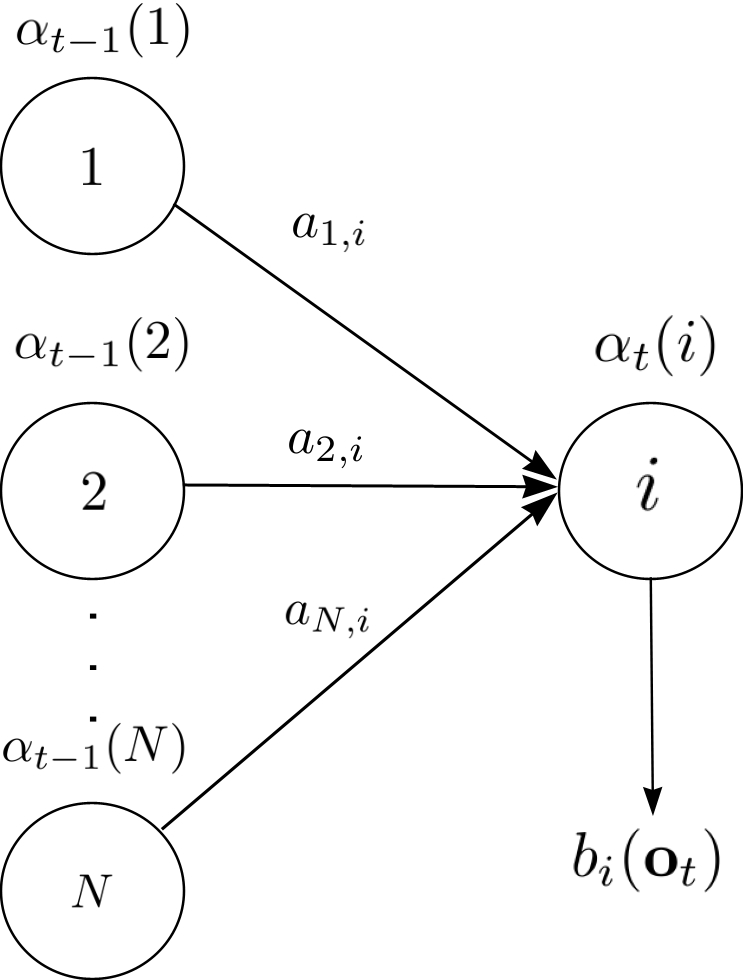
\includegraphics[width=0.8\textwidth]{forward2.jpg}
  \caption{Computation of forward probability}
  \end{figure}

\end{columns}

}

\frame{\frametitle{Forward probability}
\begin{columns}
 
\column{1.5in}
\[
 \alpha_{t}(i) \equiv
\]
\[
  P(o_{1},o_{2},\ldots, o_{t}| q_{t} = s_{i}, \lambda) = 
\]
\begin{equation}
 \label{forwardProbability}
\displaystyle \Big [ \sum_{j=1}^{N}  \alpha_{t-1}(j) a_{ij} \Big ] b_{j}(o_{t})
\end{equation}
\begin{equation}
 P({\bf O| \lambda}) = \displaystyle \sum_{i=1}^{N} \alpha_{T}(i)
\end{equation}
Problem 1 solved.
\column{2in}
  \begin{figure}
  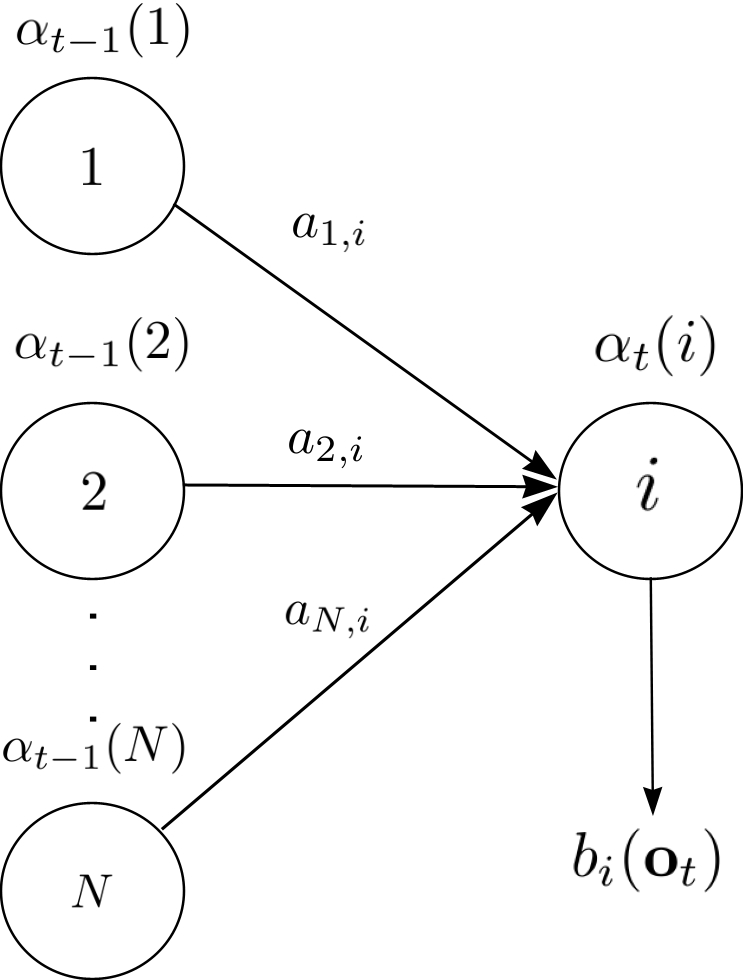
\includegraphics[width=0.8\textwidth]{forward2.jpg}
  \caption{Computation of forward probability}
  \end{figure}

\end{columns}

}

\frame{\frametitle{Learning the parameters}
  The forward-backward algorithm also commes with a backward probability:\\
 \[
  \beta_{t}(j) \equiv P(o_{t+1},o_{t+2},\ldots, o_{T}| q_{t} = s_{j}, \lambda) = 
\]
\begin{equation}
 \label{backwardProbability}
\displaystyle \sum_{i=1}^{N} a_{ij} b_{i}(o_{t+1}) \beta_{i}(o_{t+1})
\end{equation}
With this we can define the probability of being in a state at a timestep as:
\begin{equation}
 \gamma_{t}(i) \equiv (P({\bf O}|\lambda))^{-1} \alpha_{t}(i)\beta_{t}(i) 
\end{equation}
Where normalisation constant $P({\bf O}|\lambda) = \sum_{j=1}^{N} \alpha_{t}(i)\beta_{t}(i) = \sum_{j=1}^{N} \alpha_{T}(j)$.

}

\frame{\frametitle{Learning the parameters}
\[ 
\hat{a}_{ij} = frac{\text{Prob. of being in i and transfering to j}}{\text{Prob. of begin in i}} =
\]
\begin{equation}
 \hat{a}_{ij} = \frac{\displaystyle \sum_{t=1}^{T-1} \xi_{t}(i,j) } {\displaystyle \sum_{t=1}^{T-1} \gamma_{t}(i) }
\end{equation}
The priors remain fixed, for the left-to-right model.
}

\frame{\frametitle{Updating the parameters}

  Comparison with GMM:
\begin{table}
 \begin{tabular}{|l| p{3.5cm} | p{3.5cm} |}\hline
  Model:		&	{\bf GMM}		&	{\bf HMM}\\\hline
  Model parameters:	& $\lambda = \pi, \mu, \Sigma$	&	$\lambda = \pi, {\bf A}, {\bf B}$\\
  Hyper parameters:	&	Number of components	&	Topology (states, transitions), observation function\\
  Observed variables:	&	Data points		&	Observations\\
  Latent variables:	&	Priors of a component	&	State sequence\\\hline
 \end{tabular}
\end{table}

}

\frame{\frametitle{Updating parameters}

% \begin{columns}

% \column{1.5in}
% Model:\\
% Model parameters:\\
% Observed variables:\\
% Latent variables:\\
% E-step:\\
% M-step:\\
% 
% \column{1.5in}
% {\bf GMM}\\
% $\lambda = \pi, \mu, \Sigma$\\
% Data points\\
% Priors of a component\\
% Estimate the probability of a component, given the data and current parameters.\\
% Maximise $\pi$, $\mu$ and $\Sigma$.
% 
% \column{1.5in}
% {\bf HMM}\\
% $\lambda = \pi, {\bf A}, {\bf B}$\\
% Observation sequence\\
% State sequence\\
% Estimate the probability of being in a state at a timestep and the probability of transfering from a state to another state.\\
% Maximise $\pi$, ${\bf A}$ and ${\bf B}$.
% \end{columns}

\begin{table}
 \begin{tabular}{|l| p{3.5cm} | p{3.5cm} |}\hline
  Model:		&	{\bf GMM}		&	{\bf HMM}\\\hline
  E-step:		&	Estimate the probability of a component, given the data and current parameters. 
	& Estimate the probability of being in a state at a timestep and the probability of transfering from a state to another state.\\
  M-step:		& Maximise $\pi$, $\mu$ and $\Sigma$.	&	Maximise $\pi$, ${\bf A}$ and ${\bf B}$\\\hline
 \end{tabular}
\end{table}
}

\frame{\frametitle{Problems we ran into}
Consider the following observation:
  \[
   {\bf O} = \begin{pmatrix}
        -1 & 0\\
	2 & 0\\
	1 & 0\\
	-2 & 0\\
       \end{pmatrix}
  \]
}

\frame{\frametitle{Problems we ran into}
  Singularities. Consider the following observation:
  \[
   {\bf O} = \begin{pmatrix}
        -1 & 0\\
	2 & 0\\
	1 & 0\\
	-2 & 0\\
       \end{pmatrix}
  \]
  \[
   \Sigma = \begin{pmatrix}
        3\frac{1}{3} & 0\\
	0 & 0\\
       \end{pmatrix}
  \]
}
\frame{\frametitle{Problems we ran into}
 Singularities
  \[
   {\bf O} = \begin{pmatrix}
        -1 & 0\\
	2 & 0\\
	1 & 0\\
	-2 & 0\\
       \end{pmatrix}
  \]
  \[
   \Sigma = \begin{pmatrix}
        3\frac{1}{3} & 0\\
	0 & 0\\
       \end{pmatrix}
  \]
\[
 |\Sigma| = 0
\]

\begin{beamerboxesrounded}{}
\centering   Possible solution: Add some random noise.
\end{beamerboxesrounded}

}
\frame{\frametitle{Problems we ran into}
 Singularities
  \[
   {\bf O} = \begin{pmatrix}
        -1 & 0\\
	2 & 0\\
	1 & 0\\
	-2 & 0\\
       \end{pmatrix}
  \]
  \[
   \Sigma = \begin{pmatrix}
        3\frac{1}{3} & 0\\
	0 & 0\\
       \end{pmatrix}
  \]
  -> Add some random noise, also to prevent variance from collapsing.
}

\frame{\frametitle{Problems we ran into}

Short words have less likelihood.\\
Harder to recognise, more subject to writer variations.
tried to solve this by using MOG.

}
\section{Results}
\frame{\frametitle{Results on simple task}  

Simple experiment, train the model on intensity features and run it on typewritten words. Feed features from letter to both models.
\begin{table}
\caption{Results for simple typewritten words, avg over 40 runs}
 \begin{tabular}{|l|c|c|r|}\hline
    {\bf Word}   			& Letter & Number & Difference \\\hline
    LL Intensity N=6	K=1 10EM 	& 121.68 & 106.36 & 	15.32	\\
    LL All features N=6 K=1 10EM	& 795.45 & 14.08  &	781.37	\\
    LL All features N=1	K=1 10EM	& 602.22 & -90.02 &	692.22	\\
    LL All features N=6 K=3 10EM	& -186.45  &-330.14 &	143.69	\\
    LL All features N=6 K=3 30EM	& 226.96 & -820.30 &	$1.04e^{3}$\\
    LL ALL , N=6, K=1, 10EM, diagonal cov & 871.16 & 531.27 & 	487.75\\
    LL ALL , N=6, K=1, 10EM, isotropc cov & -179.00 & -272.23 &	197.35\\
    ... & ... & ...& ... \\
 \end{tabular}
\end{table}
...many many more parameters. (Interval sliding window, width of sliding window, amount of noise, ... etc.)
}

\frame{\frametitle{Results on simple task}
Step 2, take cursive words of the same length.
\begin{table}
\caption{Results for simple handwritten words, avg over 40 runs}
 \begin{tabular}{|l|c|c|r|}\hline
    {\bf Word}   			& Before & People & Difference \\\hline
    LL Intensity N=6	K=1 10EM 	& 121.68 & 106.36 & 	15.32	\\
    LL All features N=6 K=1 10EM	& 795.45 & 14.08  &	781.37	\\
    LL All features N=1	K=1 10EM	& 602.22 & -90.02 &	692.22	\\
    LL All features N=6 K=3 10EM	& -186.45  &-330.14 &	143.69	\\
    LL All features N=6 K=3 30EM	& 226.96 & -820.30 &	1.04e\^{3}\\
    LL ALL , N=6, K=1, 10EM, diagonal cov & 871.16 & 531.27 & 	487.75\\
    LL ALL , N=6, K=1, 10EM, isotropc cov & -179.00 & -272.23 &	197.35\\
    ... & ... & ...& \\
 \end{tabular}
\end{table}

}


\section{Conclusions}
\frame{\frametitle{Conclusions}  
blabla
}

\end{document}


